\chapter{Needs analysis and specification}
\section{Introduction}
In this chapter, we will describe the specification of functional and
non-functional requirements, and we will also explain how to manage the
implementation of the platform using SCRUM framework.

\section{Requirements analysis}
In this section, we will distinguish between the functional requirements that
outline the expected functionalities of our application and the non-functional
requirements to avoid the development of an unsatisfactory application.

\section{Identification of key actors}
In this section, we detail the actors who interact within our application. An
actor can be a user or a hardware device that interacts directly with the
system under study.

Our Application contains the following actors:
\begin{itemize}
      \item \textbf{Super Admin}: The super admin is the main actor who has all
            the rights to manage the platform. He has administrative rights on
            other users.
      \item \textbf{ODC Coordinator}: responsible for managing events, experts
            accounts, and other aspects of the platform.
      \item \textbf{ODC Expert}: An expert is a person with access to create
            problems and quizzes.
      \item \textbf{Participant}: A participant is a person who can solve problems
            and quizzes when participating in an event.
\end{itemize}

\section{Functional requirements}

\subsection{Actor 1: Super Admin}
\begin{itemize}
      \item \textbf{Requirement 1}: The super admin can authenticate to the
            platform.
      \item \textbf{Requirement 2}: The super admin can add an ODC coordinator.
\end{itemize}

\subsection{Actor 1: ODC Coordinator}
\begin{itemize}
      \item \textbf{Requirement 1}: the ODC coordinator can authenticate to the
            platform.
      \item \textbf{Requirement 2}: the ODC coordinator can manage ODC experts.
            \begin{itemize}
                  \item \textbf{Requirement 2.1}: the ODC coordinator can add an ODC
                        expert.
                  \item \textbf{Requirement 2.3}: the ODC coordinator can disable an
                        ODC expert.
            \end{itemize}
      \item \textbf{Requirement 3}: the ODC coordinator can manage events.
            \begin{itemize}
                  \item \textbf{Requirement 3.1}: the ODC coordinator can add an event.
                  \item \textbf{Requirement 3.2}: the ODC coordinator can edit an
                        event.
                  \item \textbf{Requirement 3.3}: the ODC coordinator can delete an
                        event.
                  \item \textbf{Requirement 3.4}: the ODC coordinator can view an
                        event.
            \end{itemize}
\end{itemize}

\subsection{Actor 1: ODC Expert}
\begin{itemize}
      \item \textbf{Requirement 1}: the ODC expert can authenticate to the
            platform.
      \item \textbf{Requirement 2}: the ODC expert can manage problems.
            \begin{itemize}
                  \item \textbf{Requirement 2.1}: the ODC expert can add a problem.
                  \item \textbf{Requirement 2.2}: the ODC expert can edit a problem.
                  \item \textbf{Requirement 2.3}: the ODC expert can delete a problem.
                  \item \textbf{Requirement 2.4}: the ODC expert can view a problem.
            \end{itemize}
      \item \textbf{Requirement 3}: the ODC expert can manage quizzes.
            \begin{itemize}
                  \item \textbf{Requirement 3.1}: the ODC expert can add a quiz.
                  \item \textbf{Requirement 3.2}: the ODC expert can edit a quiz.
                  \item \textbf{Requirement 3.3}: the ODC expert can delete a quiz.
                  \item \textbf{Requirement 3.4}: the ODC expert can view a quiz.
            \end{itemize}
\end{itemize}

\subsection{Actor 1: Participant}
\begin{itemize}
      \item \textbf{Requirement 1}: the participant can authenticate to the
            platform.
      \item \textbf{Requirement 2}: the participant can participate in an event.
            \begin{itemize}
                  \item \textbf{Requirement 2.1}: the participant can view the event
                        details.
                  \item \textbf{Requirement 2.2}: the participant can solve problems.
                  \item \textbf{Requirement 2.3}: the participant can solve quizzes.
            \end{itemize}
\end{itemize}

\section{Non-functional requirements}
The non-functional requirements consist of the technical constraints that our
application must meet, such as:

\subsection{Performance} The platform must be able to handle a large number of
concurrent users and must handle problems code execution in a reasonable time.

\subsection{Security} The platform must ensure the basic security of the
application, such as authentication, authorization add to that preventing
participants from cheating.

\section{Managing project using SCRUM}

\subsection{Teams and roles}
The Scrum team consists of a product owner, a development team, and a Scrum
Master. For our application, the roles are defined as follows in the following
figure:

\subsection{Product backlog}
A key element of any project using the Scrum method, the product backlog or
Scrum backlog must be defined and carefully maintained. What should it contain,
and how should it be constructed? Let's try to address these questions with a
simple backlog definition.

The Scrum backlog is intended to gather all the client's needs that the project
team must fulfill. It contains the list of features involved in the creation of
a product, as well as all the elements requiring the project team's
intervention. All items included in the Scrum backlog are prioritized to
indicate the order of their implementation.

\begin{longtable}{|l|p{10cm}|l|}
      \caption{Product backlog}                                                                                                \\
      \hline
      \rowcolor{blue!20} \textbf{User story id} & \textbf{User story}                                      & \textbf{Priority} \\
      \hline
      \endfirsthead

      \hline
      \rowcolor{blue!20} \textbf{User story id} & \textbf{User story}                                      & \textbf{Priority} \\
      \hline
      \endhead

      \hline
      \endfoot

      \hline
      \endlastfoot

      1                                         & as a super admin, I want to authenticate to the platform & 1                 \\ \hline
      2                                         & as a super admin, I want to logout of the platform       & 3                 \\ \hline
      3                                         & as a super admin, I want to add an ODC coordinator       & 2                 \\ \hline
      4                                         & as a super admin, I want to view ODC coordinators List   & 2                 \\ \hline
      5                                         & as a super admin, I want to view ODC Expert List         & 2                 \\ \hline
      6                                         & as a super admin, I want to disable an ODC coordinator   & 2                 \\ \hline
      7                                         & as a super admin, I want to disable an ODC Expert        & 2                 \\ \hline
      8                                         & as an ODC Coordinator, I want to connect to my account   & 2                 \\ \hline
      9                                         & as an ODC Coordinator, I want to logout of my account    & 3                 \\ \hline
      10                                        & as an ODC Coordinator, I want to update my profile       & 3                 \\ \hline
      11                                        & as an ODC Coordinator, I want to change my password      & 3                 \\ \hline
      12                                        & as an ODC Coordinator, I want to add an ODC expert       & 1                 \\ \hline
      13                                        & as an ODC Coordinator, I want to disable an ODC expert   & 2                 \\ \hline
      14                                        & as an ODC Coordinator, I want to enable an ODC expert    & 2                 \\ \hline
      15                                        & as an ODC Coordinator, I want to view ODC experts list   & 3                 \\ \hline
      16                                        & as an ODC Coordinator, I want to add an event            & 1                 \\ \hline
      17                                        & as an ODC Coordinator, I want to view all events         & 1                 \\ \hline
      18                                        & as an ODC Coordinator, I want to edit an event           & 2                 \\ \hline
      19                                        & as an ODC Coordinator, I want to delete an event         & 2                 \\ \hline
      20                                        & as an ODC Coordinator, I want to view an event           & 3                 \\ \hline
      21                                        & as an ODC Expert, I want to connect to my account        & 2                 \\ \hline
      22                                        & as an ODC Expert, I want to logout of my account         & 3                 \\ \hline
      23                                        & as an ODC Expert, I want to update my profile            & 3                 \\ \hline
      24                                        & as an ODC Expert, I want to change my password           & 3                 \\ \hline
      25                                        & as an ODC Expert, I want to add a problem                & 1                 \\ \hline
      26                                        & as an ODC Expert, I want to view all problems            & 1                 \\ \hline
      27                                        & as an ODC Expert, I want to edit a problem               & 2                 \\ \hline
      28                                        & as an ODC Expert, I want to delete a problem             & 2                 \\ \hline
      29                                        & as an ODC Expert, I want to view a problem               & 3                 \\ \hline
      30                                        & as an ODC Expert, I want to add a quiz                   & 1                 \\ \hline
      31                                        & as an ODC Expert, I want to view all quizzes             & 1                 \\ \hline
      32                                        & as an ODC Expert, I want to edit a quiz                  & 2                 \\ \hline
      33                                        & as an ODC Expert, I want to delete a quiz                & 2                 \\ \hline
      34                                        & as an ODC Expert, I want to view a quiz                  & 3                 \\ \hline
      35                                        & as a participant, I want to register to an event         & 2                 \\ \hline
      36                                        & as a participant, I want to participate in an event      & 2                 \\ \hline
\end{longtable}


\section{Sprints Planning}
The sprint planning meeting is the most important event in SCRUM. The purpose
of this meeting is to prepare the work schedule and identify the sprint
backlog. One of the outcomes of this meeting is the choice of sprint duration,
which varies depending on the project's complexity and the size of the team.


\section{Global use case diagram}
The global use case diagram is a high-level diagram that shows the interactions
between the actors and the system. It provides an overview of the system's
functionality and the actors' roles in the system.

\begin{figure}[h!]
      \centering
      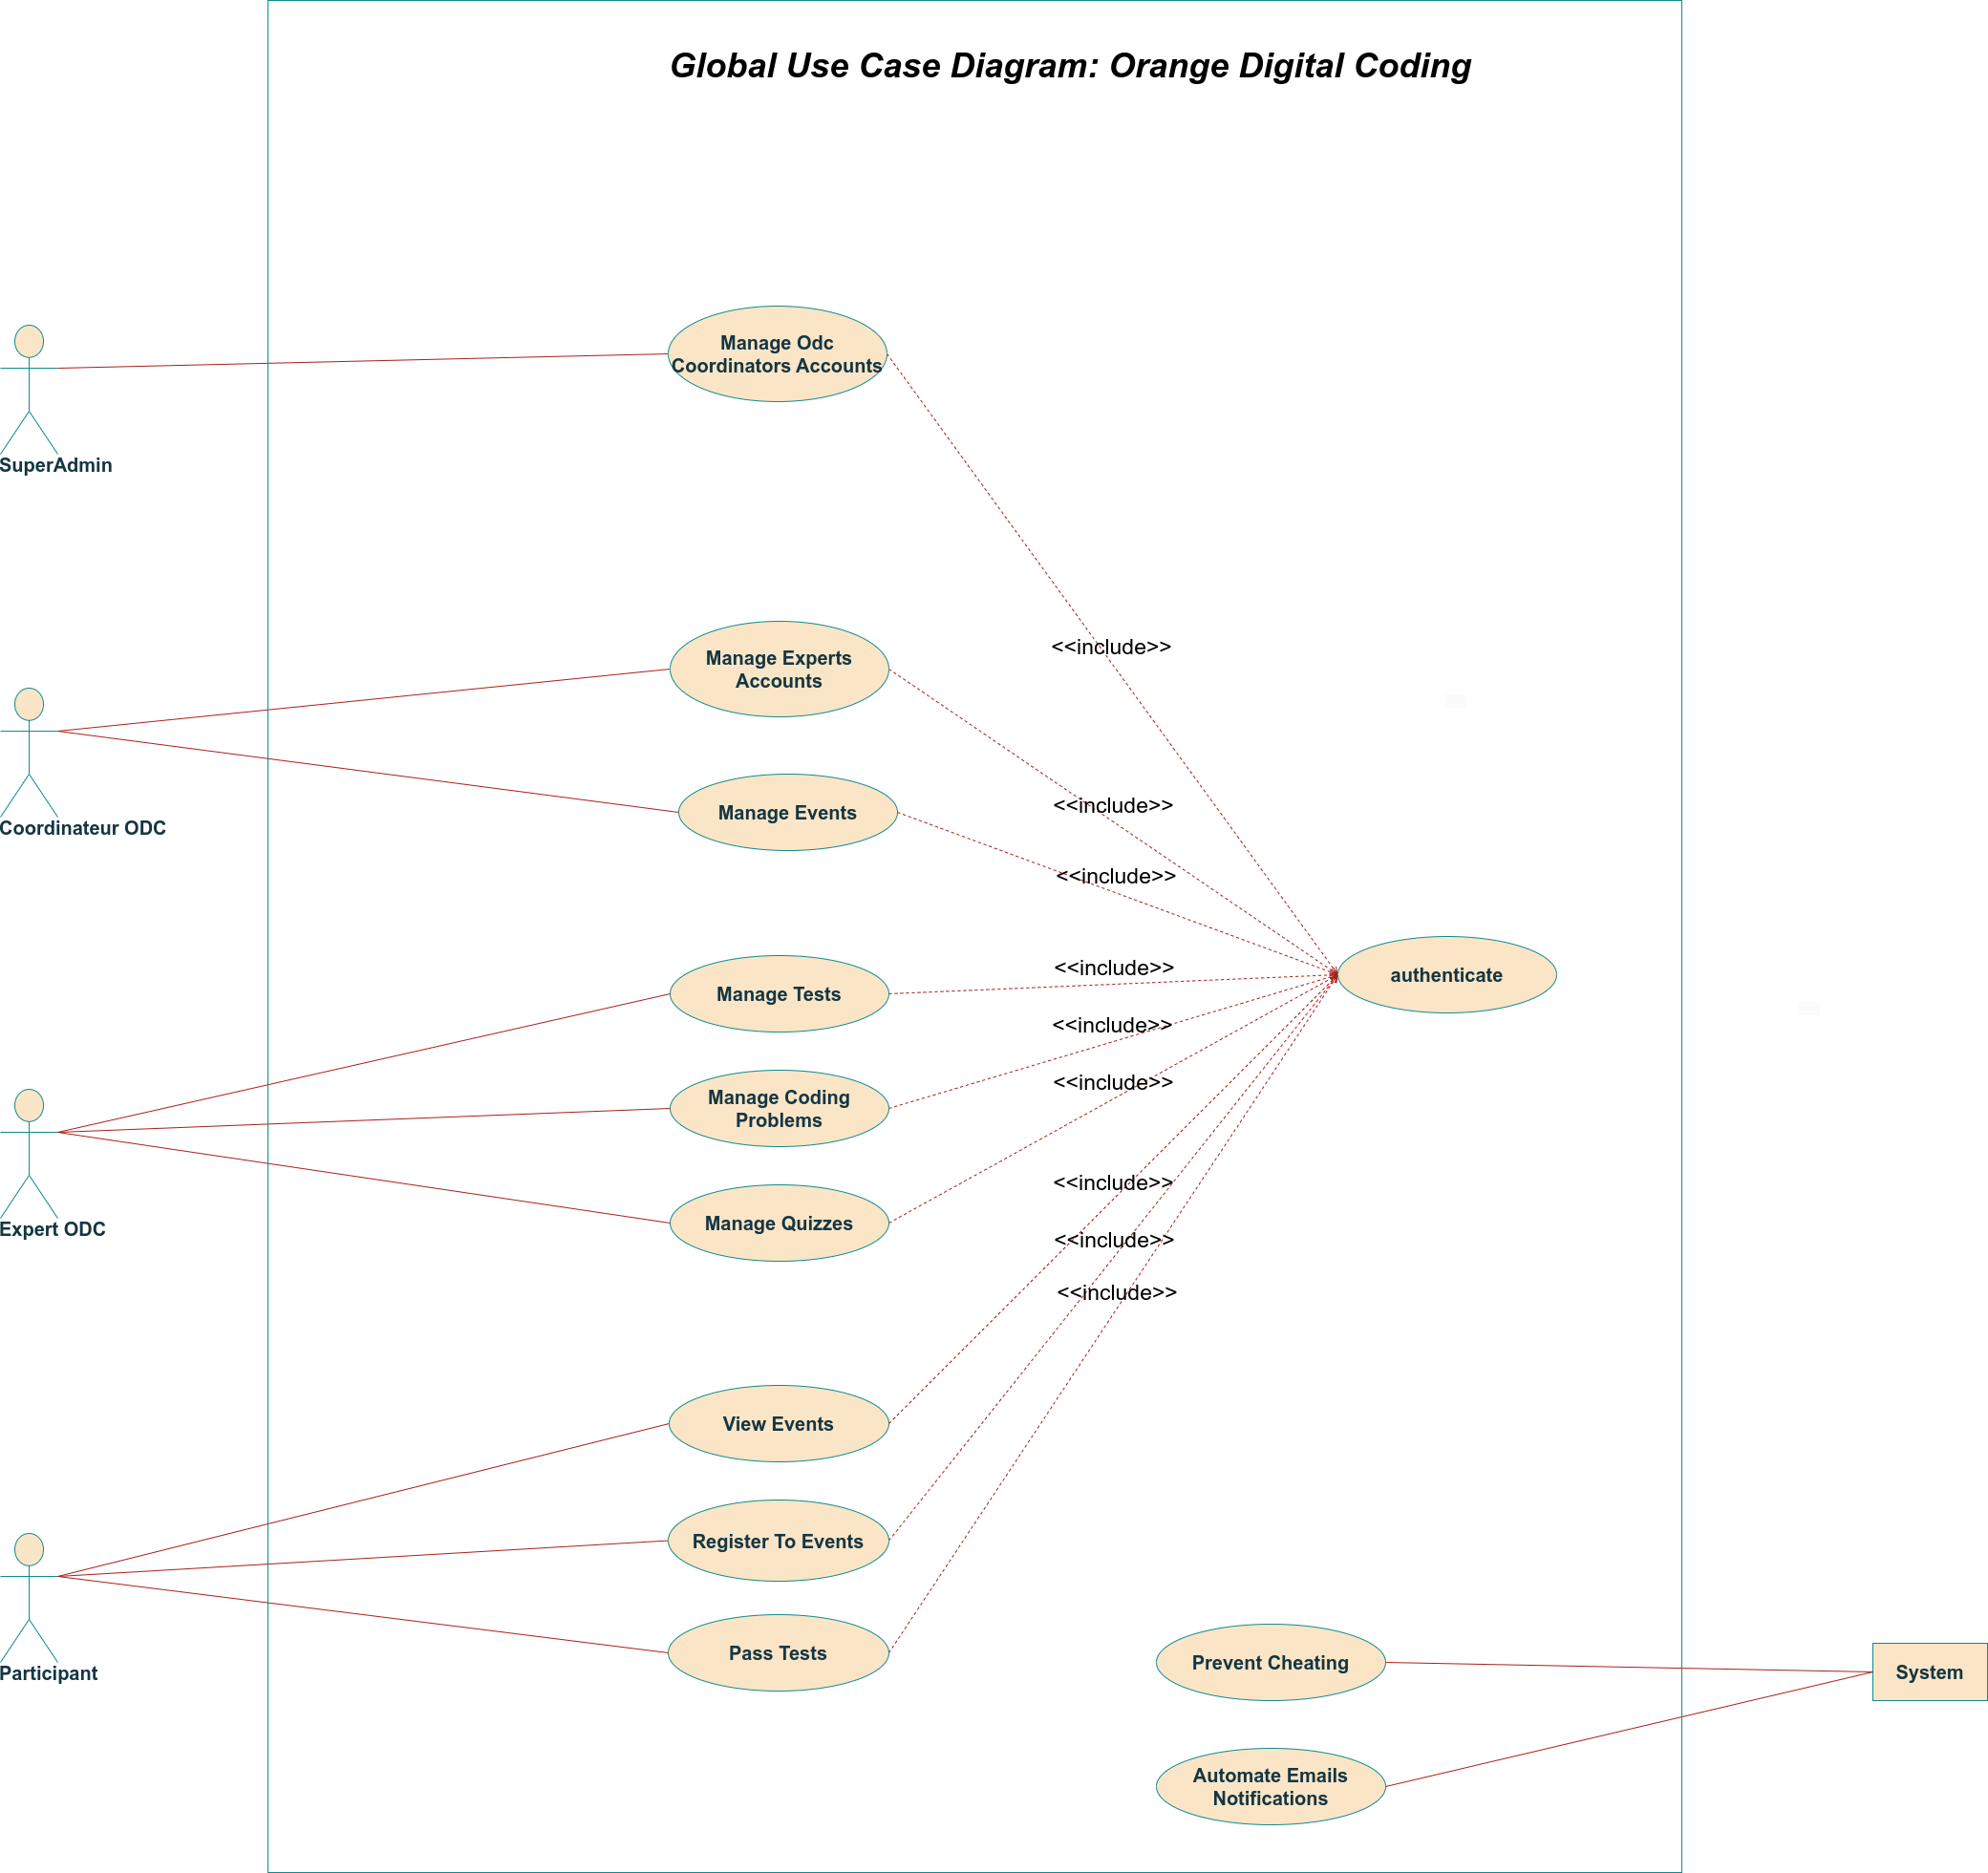
\includegraphics[height=1\textwidth, width=0.9\textwidth]{images/generalUseCase.png}
      \caption{Global use case diagram}\label{fig:use_case_diagram}
\end{figure}


\section{Database schema}
The Following figure \ref{MongoDB Schema Diagram} shows the schema of the MongoDB database used in our application.
The database contains four collections: users, events, problems, and quizzes. Each collection has a set of fields
that store the data related to that collection. The schema diagram provides a visual representation of the relationships
between the collections and the fields in each collection.


\begin{figure}[h!]
      \centering
      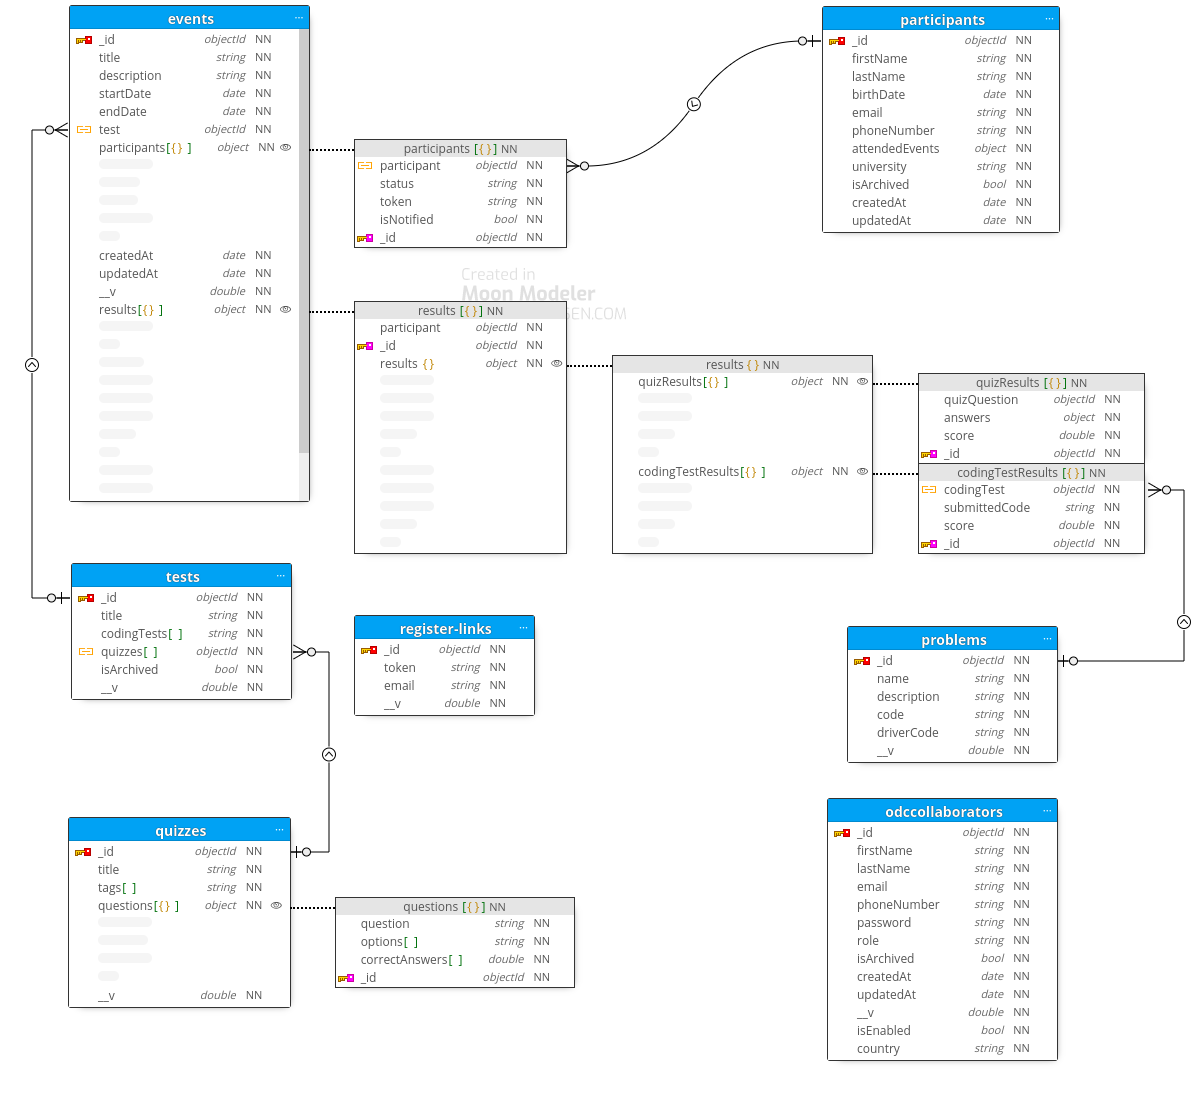
\includegraphics[width=0.9\textwidth, height=1\textwidth]{images/databaseSchema.png}
      \caption{MongoDB Schema Diagram}\label{MongoDB Schema Diagram}
\end{figure}


\section{Software and technology stack}

\subsection{Software and IDEs}
Each developer has his own preferences when it comes to choosing the right
tools for the job. Here are some of the tools we used during the development of
our application:
\subsubsection{Visual Studio Code}

Visual Studio Code is a lightweight but powerful source code editor that runs
on your desktop and is available for Windows, macOS, and Linux. It comes with
built-in support for JavaScript, TypeScript, and Node.js and has a rich
ecosystem of extensions for other languages (such as C++, C\#, Python, PHP). it really
helps to write code faster and more efficiently.
\begin{figure}[h!]
      \centering
      
\includegraphics[width=0.3\textwidth]{images/vscode.png}
      \caption{Visual Studio Code Logo}
      \label{fig:vscode}
\end{figure}

\subsubsection{Httpie}

Httpie is a command-line HTTP client that makes it easy to interact with web
services. It provides a simple and intuitive interface for sending HTTP
requests and receiving responses, making it a great tool for testing APIs and
debugging web applications.It is often introduced as the human friendly alternative to curl.

\begin{figure}[h!]
      \centering
      
\includegraphics[width=0.3\textwidth]{images/httpie.png}
      \caption{Httpie Logo}
      \label{fig:httpie}
\end{figure}


\subsubsection{Draw.io}
Draw.io is a free online diagram software for making flowcharts, process
diagrams, org charts, UML, ER and network diagrams. It is a free online diagram
software for making flowcharts, process diagrams, org charts, UML, ER and
network diagrams.
it is a great tool for creating diagrams and visual representations of
information. It is easy to use and has a wide range of features that make it
ideal for creating professional-looking diagrams.



\begin{figure}[h!]
      \centering
      
\includegraphics[width=0.3\textwidth]{images/drawio.png}
      \caption{Draw.io Logo}
      \label{fig:drawio}



\end{figure}
\newpage
\subsubsection{Slack}
Slack is a cloud-based team communication platform developed by Slack Technologies, which has been owned by Salesforce since 2020. Slack has freemium and paid subscriptions. Slack's primary userbase is businesses, and has functionalities primarily for businesses.
\begin{figure}[h!]
      \centering
      
\includegraphics[width=0.3\textwidth]{images/slack.jpg}
      \caption{Slack Logo}
      \label{fig:Slack}
\end{figure}
\subsubsection{Figma}
Figma is a collaborative web application for interface design, with additional offline features enabled by desktop applications for macOS and Windows. The feature set of Figma focuses on user interface and user experience design, with an emphasis on real-time collaboration,[1] utilising a variety of vector graphics editor and prototyping tools. The Figma mobile app for Android and iOS allows viewing and interacting with Figma prototypes in real-time on mobile and tablet devices.
Slack is a cloud-based team communication platform developed by Slack Technologies, which has been owned by Salesforce since 2020. Slack has freemium and paid subscriptions. Slack's primary userbase is businesses, and has functionalities primarily for businesses.
\begin{figure}[h!]
      \centering
      
\includegraphics[width=0.3\textwidth]{images/figma.png}
      \caption{Figma Logo}
      \label{fig:Figma}
\end{figure}

\bigbreak

\newpage
\subsection{technology stack MERN:}


\subsubsection{MongoDB}
MongoDB is a source-available cross-platform document-oriented database program.
It uses JSON-like documents with optional schemas. MongoDB is developed by
MongoDB Inc. and licensed under the Server Side Public License (SSPL).
\begin{figure}[h!]
      \centering
      
\includegraphics[width=0.3\textwidth]{images/mongodb.png}
      \caption{MongoDB Logo}
      \label{fig:mongodb}
\end{figure}

\subsubsection{Express js}
Express.js is a web application framework for Node.js, released as free
and open-source software under the MIT License. It is designed for building
web applications and APIs. It has been called the de facto standard server framework for Node.js.

\begin{figure}[h!]
      \centering
      
\includegraphics[width=0.3\textwidth]{images/Expressjs.png}
      \caption{Express Logo}
      \label{fig:express}
\end{figure}
\subsubsection{React js}
React is a JavaScript library for building user interfaces. It is maintained by
Facebook and a community of individual developers and companies. React can be
used as a base in the development of single-page or mobile applications. It is
a component-based library which is used to develop interactive UI's (User
Interfaces).

\begin{figure}[h!]
      \centering
      
\includegraphics[width=0.3\textwidth]{images/reactjs.png}
      \caption{React Logo}
      \label{fig:react}
\end{figure}



\newpage

\subsubsection{Node.js}
Node.js lets developers use JavaScript to write command line tools and for server-side scripting. The ability to run JavaScript code on the server is often used to generate dynamic web page content before the page is sent to the user's web browser. Consequently, Node.js represents a "JavaScript everywhere" paradigm,[6] unifying web-application development around a single programming language, as opposed to using different languages for the server- versus client-side programming.
\begin{figure}[h!]
      \centering
      
\includegraphics[width=0.3\textwidth]{images/node.png}
      \caption{Node.js Logo}
      \label{fig:Node.js}
\end{figure}
\bigbreak
\section{Application architecture}
We divided our project into four repositories to make it easier to manage and
maintain. Each codebase is responsible for a specific part of the application.
The project repositories are as follows:

\begin{itemize}
      \item \textbf{Dashboard front end}: This repository contains the code for the
            front end of the dashboard application. It is built using React.js and
            communicates with the back end using RESTful APIs.

      \item \textbf{Dashboard back end}: This repository is responsible for handling the
            business logic of the dashboard application. It is built using Node.js
            and Express.js and communicates with the front end using RESTful APIs.

      \item \textbf{Code execution service (Piston API)}: This is a third-party service
            that we use to execute code submitted by participants. It is built
            using Node.js and Docker and provides a secure environment for
            executing code.

      \item \textbf{Coding Problems service}: This repository contains all problems that created
            by ODC experts. It is built using Node.js and Express.js and communicates with
            the front end using RESTful APIs.
\end{itemize}


The following figure \ref{fig:architecture} shows the architecture of our application.
and how the different components interact with each other.

\begin{figure}[h!]
      \centering
      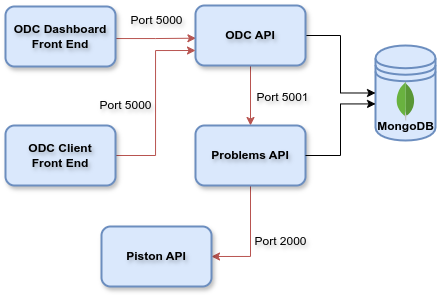
\includegraphics[width=0.7\textwidth]{images/applicationArchitecture.png}
      \caption{Application architecture}
      \label{fig:architecture}
\end{figure}